\section{Teori}

\subsection{Kondensator}
Kondensatoren kan lagre elektrisk energi i feltet sitt. Den vil lade om det er en spenningskilde tilkoblet gjennom en motstand. Den vil også utlade sin lagrede energi dersom det ikke er en tilførende kilde og komponenter den kan overføre spenning over. Det generelle uttrykket for spenning i en kondensator vil være:
\[
v_C(t) = V_{slutt} + (V_{initial} - V_{slutt})\cdot\exp\left(-(t-t_0)/\tau\right)
\]
\noindent
$\tau$ her vil være kondensatorstyrken ganget med totalresistansen, $\tau = R_{tot}\cdot C$. Det vil være en ladingsfase og en utladingsfase med kondensatorer, vi kan generalisere formlene i hvert tilfelle. I ladingsfasen har vi initialbetingelser som gir formel:
\[
\begin{aligned}
    V_{slutt} &= V_{kilde} \\
    V_{initial} &= 0 \\
    t_0 &= 0 
\end{aligned}
\]
\[
\begin{aligned}
    v_{C,opplading}(t) &= V_{slutt} + (0 - V_{slutt})\cdot\exp\left(-(t - 0)/\tau\right) \\
    v_{C,opplading}(t) &= V_{slutt} + (1 - \exp\left(-t/\tau\right))
\end{aligned}
\] 
\noindent
I utladingsfasen har vi andre initialbetingelser og vi kan utlede en formel for $v_C(t)$ i denne fasen. Her vil $t_0$ være tiden brukt i oppladingsfasen:
\[
\begin{aligned}
    V_{slutt} &= 0 \\
    V_{initial} &= v_{C,opplading}(t_0) \\
    t_0 &= t_0 \\
\end{aligned}
\]
\[
\begin{aligned}
    v_{C,nedlading}(t) &= 0 + (v_{C,opplading}(t_0) - 0)\cdot\exp\left(-(t - t_0)/\tau\right) \\
    v_{C,nedlading}(t) &= v_{C,opplading}(t_0)\cdot\exp\left(-(t - t_0)/\tau\right)
\end{aligned}
\] 

\subsection{RC - krets 1}
\begin{figure}[H]\label{fig:Krets}
\centering
\begin{circuitikz}[american voltages]

    %--- Noder (svarte prikker) ---------------------------------
    % Bunn/venstre (til jord)
    \node[circle, fill=black, inner sep=1.2pt] (G)  at (0,0)  {};
    \node[circle, fill=black, inner sep=1.2pt] (T1) at (0,5)  {}; % etter batteri oppe

    % Øvre gren
    \node[circle, fill=black, inner sep=1.2pt] (A)  at (4,5)  {};
    \node[circle, fill=black, inner sep=1.2pt] (B)  at (6,5)  {};
    \node[circle, fill=black, inner sep=1.2pt] (T2) at (10,5) {};

    % Nedre gren
    \node[circle, fill=black, inner sep=1.2pt] (BR) at (10,0) {};
    \node[circle, fill=black, inner sep=1.2pt] (F)  at (5,0)  {};
    \node[circle, fill=black, inner sep=1.2pt] (E)  at (5,2)  {};

    \node[circle, fill=black, inner sep=1.2pt] (D)  at (5,4)  {};

    %--- Labels på nodene ----------------------------------------
    \node[above] at (A) {$A$};
    \node[above] at (B) {$B$};
    \node[above right] at (E) {$E$};
    \node[below] at (F) {$F$};
    \node[right] at (D) {$D$};

    %--- Jord ----------------------------------------------------
    \draw (G) node[ground] {};

    %--- Batteri B1 ----------------------------------------------
    \draw (T1) to[battery1, l_=$B_1$, a^=$10\,\text{V}$] (G);

    %--- R1 fra batteri til A ------------------------------------
    \draw (T1) to[R, l_=$R_1$, a^=$12\,\text{k}\Omega$] (A);

    %--- Åpen bryter mellom A og B -------------------------------
    % "switch" gir en mekanisk brytersymbol
    \draw (D) to[switch] (5,5);

    %--- R2 på høyre side ----------------------------------------
    \draw (B) -- (T2)
          to[R, l_=$R_2$, a^=$27\,\text{k}\Omega$] (BR);

    %--- Nedre returledning --------------------------------------
    \draw (BR) -- (F) -- (G);

    %--- Kondensator C1 mellom E og F ----------------------------
    \draw (F) to[C, l_=$C_1$, a^=$68\,\mu\text{F}$] (E);

\end{circuitikz}
\caption{Krets for beregning av opp- og utladningsforløp}
\end{figure}



Vi skal studere kretsen i to tidsintervaller hvor bryteren i node $D$ er i $A$ og $B$. Når bryteren er tilkoblet node $A$ vil kapasitatoren lades gjennom batteriet $B_1$ og gjennomgå $R_1$ motstanden. Når bryteren er tilkoblet $B$ vil kapasitatoren utlade gjennom motstand $R_2$.

\subsubsection{Tilfelle 1}
I dette tilfellet skal $D$ til $E$ kortsluttes. Bryteren vil være mot $A$ i tidsintervallet $t \in [0,10\text{s}]$ og den med en gang etterpå tilkobles node $B$ i tidsintervallet $t \in [10\text{s}, 20\text{s}]$.

\begin{figure}[H]
\centering
\begin{circuitikz}[american voltages]

    %--- Noder (svarte prikker) ---------------------------------
    % Bunn/venstre (til jord)
    \node[circle, fill=black, inner sep=1.2pt] (G)  at (0,0)  {};
    \node[circle, fill=black, inner sep=1.2pt] (T1) at (0,5)  {}; % etter batteri oppe

    % Øvre gren
    \node[circle, fill=black, inner sep=1.2pt] (A)  at (4,5)  {};
    \node[circle, fill=black, inner sep=1.2pt] (B)  at (6,5)  {};
    \node[circle, fill=black, inner sep=1.2pt] (T2) at (10,5) {};

    % Nedre gren
    \node[circle, fill=black, inner sep=1.2pt] (BR) at (10,0) {};
    \node[circle, fill=black, inner sep=1.2pt] (F)  at (5,0)  {};
    \node[circle, fill=black, inner sep=1.2pt] (E)  at (5,2)  {};

    \node[circle, fill=black, inner sep=1.2pt] (D)  at (5,4)  {};

    %--- Labels på nodene ----------------------------------------
    \node[above] at (A) {$A$};
    \node[above] at (B) {$B$};
    \node[above right] at (E) {$E$};
    \node[below] at (F) {$F$};
    \node[right] at (D) {$D$};

    %--- Jord ----------------------------------------------------
    \draw (G) node[ground] {};

    %--- DE kortslutting

    \draw (D) to[short, -] (E);

    %--- Batteri B1 ----------------------------------------------
    \draw (T1) to[battery1, l_=$B_1$, a^=$10\,\text{V}$] (G);

    %--- R1 fra batteri til A ------------------------------------
    \draw (T1) to[R, l_=$R_1$, a^=$12\,\text{k}\Omega$] (A);

    %--- Åpen bryter mellom A og B -------------------------------
    % "switch" gir en mekanisk brytersymbol
    \draw (D) to[switch] (5,5);

    %--- R2 på høyre side ----------------------------------------
    \draw (B) -- (T2)
          to[R, l_=$R_2$, a^=$27\,\text{k}\Omega$] (BR);

    %--- Nedre returledning --------------------------------------
    \draw (BR) -- (F) -- (G);

    %--- Kondensator C1 mellom E og F ----------------------------
    \draw (F) to[C, l_=$C_1$, a^=$68\,\mu\text{F}$] (E);

\end{circuitikz}
\caption{Kretsen i tilfelle 1}
\end{figure}







\paragraph{første tidsfase. }
Siden vi her har en kortslutting fra node $D$ til $A$ kan vi forenkle kretsen som under:

\begin{figure}[H]
\centering
\begin{circuitikz}[american voltages]

    %--- Noder (svarte prikker) ---------------------------------
    % Bunn/venstre (til jord)
    \node[circle, fill=black, inner sep=1.2pt] (G)  at (0,0)  {};
    \node[circle, fill=black, inner sep=1.2pt] (T1) at (0,5)  {}; % etter batteri oppe

    % Nedre gren
    \node[circle, fill=black, inner sep=1.2pt] (F)  at (5,0)  {};

    \node[circle, fill=black, inner sep=1.2pt] (D)  at (5,5)  {};

    %--- Labels på nodene ----------------------------------------
    \node[below] at (F) {$F$};
    \node[right] at (D) {$D$};

    %--- Jord ----------------------------------------------------
    \draw (G) node[ground] {};

    %--- Batteri B1 ----------------------------------------------
    \draw (T1) to[battery1, l_=$B_1$, a^=$10\,\text{V}$] (G);

    %--- R1 fra batteri til A ------------------------------------
    \draw (T1) to[R, l_=$R_1$, a^=$12\,\text{k}\Omega$] (D);

    %--- Nedre returledning --------------------------------------
    \draw (F) -- (G);

    %--- Kondensator C1 mellom E og F ----------------------------
    \draw (F) to[C, l_=$C_1$, a^=$68\,\mu\text{F}$] (D);

\end{circuitikz}
\caption{Kretsen i tilfelle 1 i tiden $0 \le t \le 10$}
\end{figure}
\noindent
Studerer vi første fase der vi har en kapasitator som lades av $B_1$ kan vi sette opp uttrykket for spenning over tid.
\[
\begin{aligned}
    V_C(t) &= V_B (1 - \exp \left(-t/\tau\right)) \\
    V_B &= B_1 = 10\text{V} \\
    \tau &= R_1C \\
    \tau &= 12\text{k}\Omega \cdot 68 \cdot 10^{-6} \\
    \tau &= 0.816\text{s}  
\end{aligned}
\]
\noindent
Vi løser for $V_C(10)$ med de kjente verdiene våre for å få en verdi for hva spenningen kapasitatoren lagrer er etter $t=10\text{s}$.
\begin{align}
    V_C(t) &= 10 \bigl(1 - \exp\left(-t/0.816\right)\bigr) \label{eq:oppgaveAFør10} \\
    V_C(10) &= 10 \bigl(1 - \exp\left(-12.25\right)\bigr) \nonumber \\
    V_C(10) &\approx 10 \nonumber
\end{align}








\paragraph{Andre tidsfase. } Her vil vi kortslutte node $D$ til $B$ og vi kan forenkle kretsen.

\begin{figure}[H]
\centering
\begin{circuitikz}[american voltages]

    %--- Noder (svarte prikker) ---------------------------------

    % Øvre gren
    \node[circle, fill=black, inner sep=1.2pt] (T2) at (10,5) {};

    % Nedre gren
    \node[circle, fill=black, inner sep=1.2pt] (BR) at (10,0) {};
    \node[circle, fill=black, inner sep=1.2pt] (F)  at (5,0)  {};

    \node[circle, fill=black, inner sep=1.2pt] (D)  at (5,5)  {};

    %--- Labels på nodene ----------------------------------------
    \node[below] at (F) {$F$};
    \node[left] at (D) {$D$};

    %--- Jord ----------------------------------------------------
    \draw (BR) node[ground] {};

    %--- R2 på høyre side ----------------------------------------
    \draw (D) -- (T2)
          to[R, l_=$R_2$, a^=$27\,\text{k}\Omega$] (BR);

    %--- Nedre returledning --------------------------------------
    \draw (BR) -- (F);

    %--- Kondensator C1 mellom E og F ----------------------------
    \draw (D) to[V, l_=$V$, a^=$10\text{V}$] (F);

\end{circuitikz}
\caption{Kretsen i tilfelle 1}
\end{figure}

\noindent
Her er tilfelle at bryteren har umiddelbart byttet til $B$ og kapasitatoren har begynt sin utlading gjennom motstand $R_2$. $V_{start}$ vil være $V_C(10)$ fra funksjonen i første tilfelle siden dette skjer umiddelbart etterpå tilfelle 1.
\[
\begin{aligned}
    V_C(t)&=V_{start} \exp \left(-(t-10)/\tau\right) \\
    V_{start} &= 10V \\
    \tau &= R_2C \\
    \tau &= 27\text{k}\Omega \cdot 68 \cdot 10^{-6} \\
    \tau &= 1.836
\end{aligned}
\]
\noindent
Nå kan vi lage et generelt uttryk for $V_C$ etter $t = 10\text{s}$. 
\begin{equation}
    \label{eq:oppgaveAEtter10}
    V_C(t)=10\exp\left(-(t-10)/1.836\right)
\end{equation}

\paragraph{Endelig løsning}
Nå har vi to uttrykk for før og etter bryterskiftet. Denne funksjonen beskriver spenning over $DF$ på kretsen og beskriver den totale spenningen i dette området. Denne er presentert gjennom $V_{DF}$ som under. Dette er da ligning~\ref{eq:oppgaveAFør10} og ligning~\ref{eq:oppgaveAEtter10}:
\begin{equation}
V_C(t) =
\begin{cases}
10 \bigl(1 - \exp\left(-t/0.816\right)\bigr), & 0 \le t \le 10, \\
10\exp\left(-(t-10)/1.836\right) & 10 < t \le 20.
\end{cases}
\end{equation}


\subsubsection{Tilfelle 2}\label{subsec:tilfelle2iSerie}
Her er kretsen i figur~\ref{fig:Krets} modellert slik at det vil være en ny kondensator mellom node $E$ og $D$. Den har samme verdi som $C_1$. Kretsen blir seende slik ut nå:

\begin{figure}[H]
\centering
\begin{circuitikz}[american voltages]

    %--- Noder (svarte prikker) ---------------------------------
    % Bunn/venstre (til jord)
    \node[circle, fill=black, inner sep=1.2pt] (G)  at (0,0)  {};
    \node[circle, fill=black, inner sep=1.2pt] (T1) at (0,5)  {}; % etter batteri oppe

    % Øvre gren
    \node[circle, fill=black, inner sep=1.2pt] (A)  at (4,5)  {};
    \node[circle, fill=black, inner sep=1.2pt] (B)  at (6,5)  {};
    \node[circle, fill=black, inner sep=1.2pt] (T2) at (10,5) {};

    % Nedre gren
    \node[circle, fill=black, inner sep=1.2pt] (BR) at (10,0) {};
    \node[circle, fill=black, inner sep=1.2pt] (F)  at (5,0)  {};
    \node[circle, fill=black, inner sep=1.2pt] (E)  at (5,2)  {};

    \node[circle, fill=black, inner sep=1.2pt] (D)  at (5,4)  {};

    %--- Labels på nodene ----------------------------------------
    \node[above] at (A) {$A$};
    \node[above] at (B) {$B$};
    \node[above right] at (E) {$E$};
    \node[below] at (F) {$F$};
    \node[right] at (D) {$D$};

    %--- Jord ----------------------------------------------------
    \draw (G) node[ground] {};

    %--- Batteri B1 ----------------------------------------------
    \draw (T1) to[battery1, l_=$B_1$, a^=$10\,\text{V}$] (G);

    %--- R1 fra batteri til A ------------------------------------
    \draw (T1) to[R, l_=$R_1$, a^=$12\,\text{k}\Omega$] (A);

    %--- Åpen bryter mellom A og B -------------------------------
    % "switch" gir en mekanisk brytersymbol
    \draw (D) to[switch] (5,5);

    %--- R2 på høyre side ----------------------------------------
    \draw (B) -- (T2)
          to[R, l_=$R_2$, a^=$27\,\text{k}\Omega$] (BR);

    %--- Nedre returledning --------------------------------------
    \draw (BR) -- (F) -- (G);

    %--- Kondensator C1 mellom E og F ----------------------------
    \draw (F) to[C, l_=$C_1$, a^=$68\,\mu\text{F}$] (E);

    %--- Kondensator C1 mellom D og E ----------------------------
    \draw (E) to[C, l_=$C_2$, a^=$68\,\mu\text{F}$] (D);

\end{circuitikz}
\caption{Krets for beregning av opp- og utladningsforløp}
\end{figure}

I denne kretsen kan vi beskrive de ulike spenningene over $DF$. Det vil være én spenning over $C_1$, én over $C_2$ og vi kan også beskrive spenningen over hele $DF$. Siden disse er i seriekobling og strømmen vil være like over $DF$ og både $C_1$ og $C_2$ er like kan vi se at spenningen over dem må være lik:
\[
\begin{aligned}
    i_{EF} &= C_1\frac{dv_{C1}}{dt} \\
    i_{DE} &= C_2\frac{dv_{C2}}{dt} \\
    i_{EF} = i_{DE} \quad &\text{og} \quad C_1 = C_2 \\
    \frac{dv_{C1}}{dt} &= \frac{dv_{C2}}{dt}
\end{aligned}
\]
\noindent
Kan vi konkludere med at spenningene må være like.
\[
v_{C1}(t) = v_{C2}(t), \qquad \text{for alle $t$}
\]
\noindent
Og vi har uttryk for alle spenningene på skinnen $DF$:
\[
\begin{aligned}
    v_{C1}(t) &= v_{C2}(t) = v_{C}(t) \\
    V_{DF}(t) &= v_{C1}(t) + v_{C2}(t) \\
    V_{DF}(t) &= 2v_{C}(t)
\end{aligned}
\]
\noindent
Nå kan vi se på prosessen der bryteren står i $A$ og når bryteren står i $B$. Som i tilfelle 1 vil det være en ladeprosess og en utladeprosess. Dette er definert ved lading i tida $t \in [0, 10\text{s}]$ og utlading i tidsrommet $t \in [10\text{s}, 20\text{s}]$. Vi må også behandle $C_1$ og $C_2$ som én totalkapasitator. Da må vi finne totalkapasitansen sett fra $DF$. $C_{tot}$ blir: $\left(C_{tot}\right)^{-1} = \left(C_1\right)^{-1} + \left(C_2\right)^{-1} \rightarrow C_{tot} = 34 \mu\text{F}$. 

\paragraph{Ladeprosess. } Her har vi en kortslutting fra $D$ til $A$.

\begin{figure}[H]
\centering
\begin{circuitikz}[american voltages]

    %--- Noder (svarte prikker) ---------------------------------
    % Bunn/venstre (til jord)
    \node[circle, fill=black, inner sep=1.2pt] (G)  at (0,0)  {};
    \node[circle, fill=black, inner sep=1.2pt] (T1) at (0,5)  {}; % etter batteri oppe

    % Nedre gren
    \node[circle, fill=black, inner sep=1.2pt] (F)  at (5,0)  {};

    \node[circle, fill=black, inner sep=1.2pt] (D)  at (5,5)  {};

    \node[circle, fill=black, inner sep=1.2pt] (E)  at (5, 2.5)  {};

    %--- Labels på nodene ----------------------------------------
    \node[below] at (F) {$F$};
    \node[right] at (D) {$D$};
    \node[right] at (E) {$E$};

    %--- Jord ----------------------------------------------------
    \draw (G) node[ground] {};

    %--- Batteri B1 ----------------------------------------------
    \draw (T1) to[battery1, l_=$B_1$, a^=$10\,\text{V}$] (G);

    %--- R1 fra batteri til A ------------------------------------
    \draw (T1) to[R, l_=$R_1$, a^=$12\,\text{k}\Omega$] (D);

    %--- Nedre returledning --------------------------------------
    \draw (F) -- (G);

    %--- Kondensator C1 mellom E og F ----------------------------
    \draw (F) to[C, l_=$C_1$, a^=$68\,\mu\text{F}$] (E);

    %--- Kondensator C1 mellom E og D ----------------------------
    \draw (E) to[C, l_=$C_2$, a^=$68\,\mu\text{F}$] (D);

\end{circuitikz}
\caption{Kretsen i tilfelle 1 i tiden $0 \le t \le 10$}
\end{figure}

\noindent
Vi finner \emph{tau} og uttrykket for $V_{DF}(t)$ fra sekund $0$ til $10$:
\[
\begin{aligned}
    \tau &= R_1 C_{tot} \\
    \tau &= 12\text{k}\Omega \cdot 34 \cdot 10^{-6} \\
    \tau &= 0.408\text{s} \\
    V_{DF}(t) &= V_B (1 - \exp \left(-t/\tau\right)) \\
    V_{DF}(t) &= 10 (1 - \exp \left(-t/0.408\right))
\end{aligned}
\]
Her vil uttrykket for spenningen i den enkelte kapasitatoren være $v_{Cn}(t) = \frac{1}{2}V_{DF}(t)$.






\paragraph{Utladeprosess. } Her vil vi kortslutte fra $D$ til $B$.
\begin{figure}[H]
\centering
\begin{circuitikz}[american voltages]

    %--- Noder (svarte prikker) ---------------------------------

    % Øvre gren
    \node[circle, fill=black, inner sep=1.2pt] (T2) at (10,5) {};

    % Nedre gren
    \node[circle, fill=black, inner sep=1.2pt] (BR) at (10,0) {};
    \node[circle, fill=black, inner sep=1.2pt] (F)  at (5,0)  {};

    \node[circle, fill=black, inner sep=1.2pt] (D)  at (5,5)  {};
    \node[circle, fill=black, inner sep=1.2pt] (E) at (5, 2.5) {};

    %--- Labels på nodene ----------------------------------------
    \node[below] at (F) {$F$};
    \node[left] at (D) {$D$};
    \node[left] at (E) {$E$};

    %--- Jord ----------------------------------------------------
    \draw (BR) node[ground] {};

    %--- R2 på høyre side ----------------------------------------
    \draw (D) -- (T2)
          to[R, l_=$R_2$, a^=$27\,\text{k}\Omega$] (BR);

    %--- Nedre returledning --------------------------------------
    \draw (BR) -- (F);

    %--- Kondensator C1 mellom F og E ----------------------------
    \draw (E) to[V, l_=$V_1$, a^=$5\text{V}$] (F);

    %--- Kondensator C1 mellom E og D ----------------------------
    \draw (D) to[V, l_=$V_2$, a^=$5\text{V}$] (E);

\end{circuitikz}
\caption{Kretsen i tilfelle 2}
\end{figure}
\noindent
Utregning for $V_{DF}(t)$ innebærer å vite $V_{DF}|_{t1}(10)$. Denne er da $\left(\approx 10\right)$. $V_{DF}(t)$ for denne utladeprosessen er som under.
\[
\begin{aligned}
    \tau &= R_2 C_{tot} \\
    \tau &= 27\text{k}\Omega \cdot 34 \cdot 10^{-6} \\
    \tau &= 0.918\text{s} \\
    V_{DF}(t) &= 10 \exp \left(-(t - 10)/0.918\right)
\end{aligned}
\]

\paragraph{Endelig uttrykk. }
\[
V_{DF}(t) = \begin{cases}
    10\left(1 - \exp \left(-t / 0.408\right)\right), 0 \le t \le 10, \\ 10\exp\left(-(t - 10)/0.918\right), 10 \le t \le 20 
\end{cases}
\]
\[
v_{C1}(t) = v_{C2}(t) = \begin{cases}
    5\left(1 - \exp \left(-t / 0.408\right)\right), 0 \le t \le 10, \\ 5\exp\left(-(t - 10)/0.918\right), 10 \le t \le 20 
\end{cases}
\]


\subsubsection{Tilfelle 3}
Her skal vi kortslutte $DE$ og parallelkoble $C_2$ med $C_1$ mellom $FE$. Kretsen blir nå seende slik ut:

\begin{figure}[H]
\centering
\begin{circuitikz}[american voltages]

    %--- Noder (svarte prikker) ---------------------------------
    % Bunn/venstre (til jord)
    \node[circle, fill=black, inner sep=1.2pt] (G)  at (0,0)  {};
    \node[circle, fill=black, inner sep=1.2pt] (T1) at (0,5)  {}; % etter batteri oppe

    % Øvre gren
    \node[circle, fill=black, inner sep=1.2pt] (A)  at (4,5)  {};
    \node[circle, fill=black, inner sep=1.2pt] (B)  at (6,5)  {};
    \node[circle, fill=black, inner sep=1.2pt] (T2) at (10,5) {};

    % Nedre gren
    \node[circle, fill=black, inner sep=1.2pt] (BR) at (10,0) {};
    \node[circle, fill=black, inner sep=1.2pt] (F)  at (5,0)  {};
    \node[circle, fill=black, inner sep=1.2pt] (FL)  at (3,0)  {};
    \node[circle, fill=black, inner sep=1.2pt] (FR)  at (7,0)  {};
    \node[circle, fill=black, inner sep=1.2pt] (E)  at (5,2)  {};
    \node[circle, fill=black, inner sep=1.2pt] (EL)  at (3,2)  {};
    \node[circle, fill=black, inner sep=1.2pt] (ER)  at (7,2)  {};

    \node[circle, fill=black, inner sep=1.2pt] (D)  at (5,4)  {};

    %--- Labels på nodene ----------------------------------------
    \node[above] at (A) {$A$};
    \node[above] at (B) {$B$};
    \node[above right] at (E) {$E$};
    \node[below] at (F) {$F$};
    \node[right] at (D) {$D$};

    %--- Jord ----------------------------------------------------
    \draw (G) node[ground] {};

    %--- DE kortslutting

    \draw (D) to[short, -] (E);

    %--- Batteri B1 ----------------------------------------------
    \draw (T1) to[battery1, l_=$B_1$, a^=$10\,\text{V}$] (G);

    %--- R1 fra batteri til A ------------------------------------
    \draw (T1) to[R, l_=$R_1$, a^=$12\,\text{k}\Omega$] (A);

    %--- Åpen bryter mellom A og B -------------------------------
    % "switch" gir en mekanisk brytersymbol
    \draw (D) to[switch] (5,5);

    %--- R2 på høyre side ----------------------------------------
    \draw (B) -- (T2)
          to[R, l_=$R_2$, a^=$27\,\text{k}\Omega$] (BR);

    %--- Nedre returledning --------------------------------------
    \draw (BR) -- (F) -- (G);

    \draw (EL) -- (E) -- (ER);

    %--- Kondensator C1 mellom E og F ----------------------------
    \draw (FL) to[C, l_=$C_1$, a^=$68\,\mu\text{F}$] (EL);
    \draw (FR) to[C, l_=$C_2$, a^=$68\,\mu\text{F}$] (ER);

\end{circuitikz}
\caption{Kretsen i tilfelle 3 med parallellkoblede kondensatorer $C_1$ og $C_2$}
\end{figure}

\noindent
Vi skal gjenta beregninger for samme mål som i tilfelle 1 og 2. Altså, en ladeperiode og utladeperiode i samme tidsrom som tidligere. Forskjellen her er at spenningen over $DF$ vil være representert av to kapasitatorer i parallell. Nå kan $C_{tot}$ regnes ut som
\[
C_{tot} = C_1 + C_2 \;\;\Rightarrow\;\; C_{tot} = 136\,\mu\text{F}.
\]
Over identiske komponenter vil strømmen fordeles, men spenningen over begge kondensatorene vil være den samme, siden de er parallellkoblet:
\[
v_{C1}(t) = v_{C2}(t) = V_{DF}(t).
\]
Vi ser på lade- og utladeperioden.

\paragraph{Ladeperiode. } Her vil kretsen simplifiseres til.
\begin{figure}[H]
\centering
\begin{circuitikz}[american voltages]

    %--- Noder (svarte prikker) ---------------------------------
    % Bunn/venstre (til jord)
    \node[circle, fill=black, inner sep=1.2pt] (G)  at (0,0)  {};
    \node[circle, fill=black, inner sep=1.2pt] (T1) at (0,5)  {}; % etter batteri oppe

    % Nedre gren
    \node[circle, fill=black, inner sep=1.2pt] (F)  at (5,0)  {};
    \node[circle, fill=black, inner sep=1.2pt] (FL)  at (3,0)  {};
    \node[circle, fill=black, inner sep=1.2pt] (FR)  at (7,0)  {};
    \node[circle, fill=black, inner sep=1.2pt] (E)  at (5,2)  {};
    \node[circle, fill=black, inner sep=1.2pt] (EL)  at (3,2)  {};
    \node[circle, fill=black, inner sep=1.2pt] (ER)  at (7,2)  {};

    \node[circle, fill=black, inner sep=1.2pt] (D)  at (5,5)  {};

    %--- Labels på nodene ----------------------------------------
    \node[above right] at (E) {$E$};
    \node[below] at (F) {$F$};
    \node[right] at (D) {$D$};

    %--- Jord ----------------------------------------------------
    \draw (G) node[ground] {};

    %--- DE kortslutting

    \draw (D) to[short, -] (E);

    %--- Batteri B1 ----------------------------------------------
    \draw (T1) to[battery1, l_=$B_1$, a^=$10\,\text{V}$] (G);

    %--- R1 fra batteri til A ------------------------------------
    \draw (T1) to[R, l_=$R_1$, a^=$12\,\text{k}\Omega$] (D);

    %--- Nedre returledning --------------------------------------
    \draw (G) -- (FR);

    \draw (EL) -- (E) -- (ER);

    %--- Kondensator C1 mellom E og F ----------------------------
    \draw (FL) to[C, l_=$C_1$, a^=$68\,\mu\text{F}$] (EL);
    \draw (FR) to[C, l_=$C_2$, a^=$68\,\mu\text{F}$] (ER);

\end{circuitikz}
\caption{Forenklet krets for ladeperioden i tilfelle 3, $0 \le t \le 10\,\text{s}$}
\end{figure}

\noindent
Her ser vi en spenningskilde $B_1$ som lader opp en ekvivalent kapasitans $C_{tot}$ via motstanden $R_1$. Tidskonstanten og spenningen over $DF$ i ladeperioden blir
\[
\begin{aligned}
    \tau &= R_1 C_{tot} \\
         &= 12\text{k}\Omega \cdot 136 \cdot 10^{-6} \\
         &= 1.632\,\text{s}, \\[0.5em]
    V_{DF}(t) &= V_B\bigl(1 - \exp(-t/\tau)\bigr) \\
              &= 10\bigl(1 - \exp(-t/1.632)\bigr), \qquad 0 \le t \le 10.
\end{aligned}
\]
Siden kondensatorene er parallellkoblet, har vi
\[
v_{C1}(t) = v_{C2}(t) = V_{DF}(t), \qquad 0 \le t \le 10.
\]

\noindent
Når $t = 10\,\text{s}$ er det gått flere tidskonstanter, og vi kan ta
\[
V_{DF}(10) \approx 10\,\text{V}.
\]









\paragraph{Utladeperiode. } Kretsen blir seende slik ut:

\begin{figure}[H]
\centering
\begin{circuitikz}[american voltages]

    \node[circle, fill=black, inner sep=1.2pt] (T2) at (10,5) {};

    % Nedre gren
    \node[circle, fill=black, inner sep=1.2pt] (BR) at (10,0) {};
    \node[circle, fill=black, inner sep=1.2pt] (F)  at (5,0)  {};
    \node[circle, fill=black, inner sep=1.2pt] (FL)  at (3,0)  {};
    \node[circle, fill=black, inner sep=1.2pt] (FR)  at (7,0)  {};
    \node[circle, fill=black, inner sep=1.2pt] (E)  at (5,2)  {};
    \node[circle, fill=black, inner sep=1.2pt] (EL)  at (3,2)  {};
    \node[circle, fill=black, inner sep=1.2pt] (ER)  at (7,2)  {};

    \node[circle, fill=black, inner sep=1.2pt] (D)  at (5,5)  {};

    %--- Labels på nodene ----------------------------------------
    \node[above right] at (E) {$E$};
    \node[below] at (F) {$F$};
    \node[left] at (D) {$D$};

    %--- Jord ----------------------------------------------------
    \draw (BR) node[ground] {};

    %--- DE kortslutting

    \draw (D) to[short, -] (E);

    %--- R2 på høyre side ----------------------------------------
    \draw (D) -- (T2)
          to[R, l_=$R_2$, a^=$27\,\text{k}\Omega$] (BR);

    %--- Nedre returledning --------------------------------------
    \draw (FL) -- (BR);

    \draw (EL) -- (E) -- (ER);

    %--- Kondensator C1 mellom E og F ----------------------------
    \draw (FL) to[V, l_=$V_1$, a^=$10\text{V}$] (EL);
    \draw (FR) to[V, l_=$V_2$, a^=$10\text{V}$] (ER);

\end{circuitikz}
\caption{Kretsen i tilfelle 3 med parallellkoblede kondensatorer $C_1$ og $C_2$}
\end{figure}


\noindent
Når bryteren umiddelbart etterpå kobles til node $B$, vil de to parallellkoblede kondensatorene utlades gjennom motstanden $R_2$ på samme måte som én kapasitans $C_{tot}$.

\noindent
For utladingen i tidsintervallet $t \in [10\,\text{s}, 20\,\text{s}]$ får vi
\[
\begin{aligned}
    \tau &= R_2 C_{tot} \\
         &= 27\text{k}\Omega \cdot 136 \cdot 10^{-6} \\
         &= 3.672\,\text{s}, \\[0.5em]
    V_{DF}(t) &= V_{DF}(10)\,\exp\bigl(-(t-10)/\tau\bigr) \\
              &\approx 10\,\exp\left(-(t-10)/3.672\right), \qquad 10 \le t \le 20.
\end{aligned}
\]
Igjen er spenningen over hver av kondensatorene lik spenningen over $DF$:
\[
v_{C1}(t) = v_{C2}(t) = V_{DF}(t), \qquad 10 \le t \le 20.
\]

\paragraph{Endelig uttrykk. }
Vi kan nå samle resultatene for hele tidsintervallet:
\[
V_{DF}(t) =
\begin{cases}
10\bigl(1 - \exp(-t/1.632)\bigr), & 0 \le t \le 10, \\
10\exp\left(-(t-10)/3.672\right), & 10 \le t \le 20,
\end{cases}
\]
og spenningen over hver av kondensatorene er
\[
v_{C1}(t) = v_{C2}(t) = V_{DF}(t).
\]

\subsubsection{Grafen for hvert tilfelle.}

\begin{figure}[H]
\centering
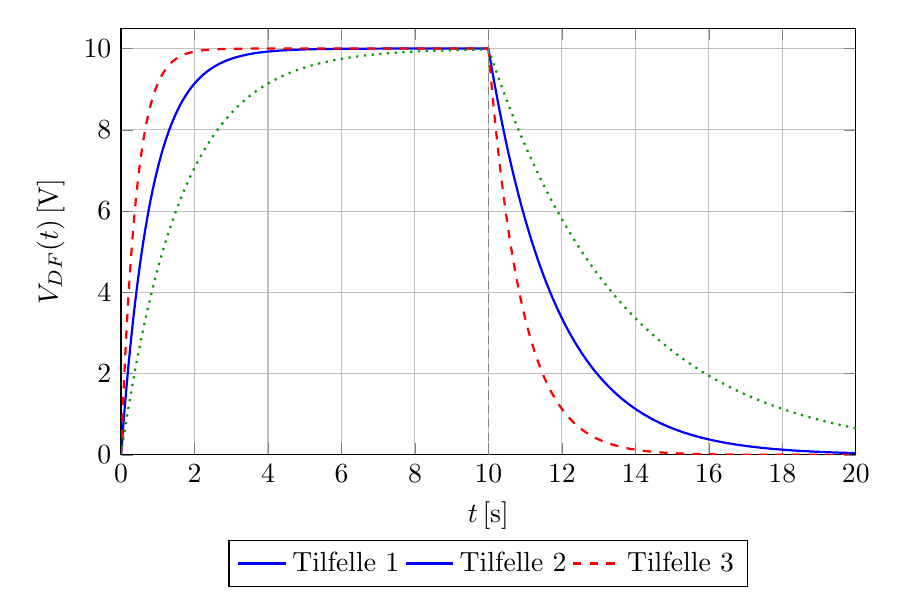
\begin{tikzpicture}
\begin{axis}[
    width=0.9\textwidth,
    height=7cm,
    xlabel={$t\,[\mathrm{s}]$},
    ylabel={$V_{DF}(t)\,[\mathrm{V}]$},
    xmin=0, xmax=20,
    ymin=0, ymax=10.5,
    grid=both,
    legend style={at={(0.5,-0.2)},anchor=north,legend columns=3},
    samples=200
]

    % --- Tilfelle 1: enkel kondensator (tau = 0.816 og 1.836) ---
    % Lading 0–10 s
    \addplot[
        thick,
        blue,
        domain=0:10
    ]
        {10*(1 - exp(-x/0.816))};

    % Utlading 10–20 s
    \addplot[
        thick,
        blue,
        domain=10:20
    ]
        {10*exp(-(x-10)/1.836)};

    \addlegendentry{Tilfelle 1}

    % --- Tilfelle 2: serie (C_tot = 34 µF, tau = 0.408 og 0.918) ---
    % Lading 0–10 s
    \addplot[
        thick,
        red,
        dashed,
        domain=0:10
    ]
        {10*(1 - exp(-x/0.408))};

    % Utlading 10–20 s
    \addplot[
        thick,
        red,
        dashed,
        domain=10:20
    ]
        {10*exp(-(x-10)/0.918)};

    \addlegendentry{Tilfelle 2}

    % --- Tilfelle 3: parallell (C_tot = 136 µF, tau = 1.632 og 3.672) ---
    % Lading 0–10 s
    \addplot[
        thick,
        green!60!black,
        dotted,
        domain=0:10
    ]
        {10*(1 - exp(-x/1.632))};

    % Utlading 10–20 s
    \addplot[
        thick,
        green!60!black,
        dotted,
        domain=10:20
    ]
        {10*exp(-(x-10)/3.672)};

    \addlegendentry{Tilfelle 3}

    % Vertikal linje ved bryterskift t = 10 s (valgfritt)
    \addplot[
        gray,
        densely dashed
    ]
        coordinates {(10,0) (10,10.5)};

\end{axis}
\end{tikzpicture}
\caption{Spenning $V_{DF}(t)$ for tilfelle 1--3 i tidsrommet $0 \le t \le 20\,\mathrm{s}$.}
\end{figure}





\subsection{RC - krets 2}

\begin{figure}[H]
\centering
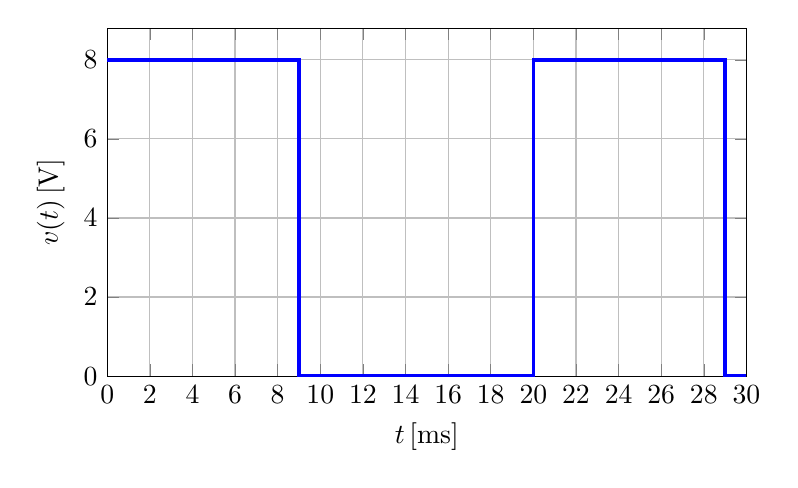
\begin{tikzpicture}
\begin{axis}[
    width=0.8\textwidth,
    height=6cm,
    xlabel={$t\,[\mathrm{ms}]$},
    ylabel={$v(t)\,[\mathrm{V}]$},
    xmin=0, xmax=30,
    ymin=0, ymax=8.8,
    ytick={0,2,4,6,8},
    xtick={0,2,...,30},
    grid=both
]
    \addplot[const plot, very thick, blue]
        coordinates {
            (0,8)
            (9,8)
            (9,0)
            (20,0)
            (20,8)
            (29,8)
            (29,0)
            (30,0)
        };
\end{axis}
\end{tikzpicture}
\caption{Inngangssignal $v(t)$ med høy-nivå $8\,\mathrm{V}$ i 9\,ms per periode.}
\end{figure}



\begin{figure}[H]
\centering
\begin{circuitikz}[american voltages]

    \node[circle, fill=black, inner sep=1.2pt] (BL)  at (0, 0)  {};
    \node[circle, fill=black, inner sep=1.2pt] (B)  at (5, 0)  {};
    \node[circle, fill=black, inner sep=1.2pt] (BR)  at (10, 0)  {};
    \node[circle, fill=black, inner sep=1.2pt] (TL)  at (0, 5)  {};
    \node[circle, fill=black, inner sep=1.2pt] (T)  at (5, 5)  {};
    \node[circle, fill=black, inner sep=1.2pt] (TR)  at (10, 5)  {};
    \node[circle, draw=black, fill=none, thick, inner sep=2pt] (VT)  at (12, 4)  {};
    \node[circle, draw=black, fill=none, thick, inner sep=2pt] (VB)  at (12, 1)  {};


    \node[above] at (T) {$A$};
    \node[ground] at (B) {};

    \node at (12, 3.5) {$+$};
    \node at (12, 1.5) {$-$};
    \node at (12, 2.5) {$v_0(t)$};

    \draw (TL) to[V=$v(t)$] (BL);
    \draw (TL) to[R=$2.2\text{k}\Omega$] (T);
    \draw (T) to[R=$3.9\text{k}\Omega$] (TR);
    \draw (TR) to[R, l_=$3.3\text{k}\Omega$] (BR);
    \draw (T) to[C, l_=$v_C(t)$, a^=$1\mu\text{F}$] (B);
    \draw (BL) -- (BR);

    \draw (10, 4) to[short, -] (VT);
    \draw (10, 1) to[short, -] (VB);
    


\end{circuitikz}
\caption{Kretsen i tilfelle 1}
\end{figure}



\subsubsection{DutyCycle, frekvens og symmetrilinje}
Ser vi på grafen i figur \ref{IKKEDERENDA} kan vi trekke ut DutyCycle, frekvens og symmetrilinje. Definisjonene deres er som følger:
\[
\begin{aligned}
    DutyCycle &= \frac{T_{topp}}{T_{periode}} \\
    f &= \frac{1}{T_{periode}} \\
    V_{symmetri} &= \frac{V_{min} + V_{maks}}{2}
\end{aligned}
\]
\noindent
Analyserer vi grafen ser vi at perioden er $20\text{ms}$, fordi kurven har samme tilstand, verdi og retning i enhver punkt på grafen med $20\text{ms}$ i avstand. Dette er da $T_{periode}$. Vi ser også at tiden grafen er på sin $V_{maks}$ er $9\text{ms}$. Dette er da $T_{topp}$. Grafens $V_{min}$ og $V_{maks}$ er henholdsvis $0\text{V}$ og $8\text{V}$. Da som vi har verdier løser vi for DutyCycle, frekvens og symmetrilinje under:
\[
\begin{aligned}
    T_{periode} = 20\text{ms}, \quad T_{topp} = 9\text{ms}, & \quad V_{min} = 0\text{V}, \quad V_{maks} = 8\text{V} \\
    DutyCycle &= \frac{9\text{ms}}{20\text{ms}} = 0.45 = 45\% \\
    f &= \frac{1}{20\text{ms}} = 50 \text{Hz} \\
    V_{sym} &= \frac{0\text{V} + 8\text{V}}{2} = 4\text{V}
\end{aligned}
\]

\subsubsection{$v_C(t)$ og $v_0(t)$ i kretsen}
Først kan vi finne maksimal spenning i node $A$ over kondensatoren. Inngangsspenningen vil produsere en spenning lik $V_{max}$ som betyr at når $v(t) = 8\text{V}$ har stått på lenge vil kondensatoren være i likespenningstilstand. Sett fra spenningskilden ligger alle motstandene i serie til jord. Dermed kan vi regne $R_{last}$ etter node $A$. Og dermed vil maksimumsspenningen i node $A$ kunne uttrykkes som:
\[
\begin{aligned}
    R_{last} &= \left(3.9 + 3.3\right){k}\Omega \\
    R_{last} &= 7.2\text{k}\Omega
\end{aligned}
\]

\[
\begin{aligned}
    V_{A,max} &= V_{C}^{max} = 8\text{V}\cdot\frac{R_{last}}{2.2\text{k}\Omega+R_{last}} \\
    V_{A,max} &\approx 6.1\text{V}
\end{aligned}
\]

\noindent
Dette er den maksimale spenningen kondensatoren kan få hvis den får "uendelig" tid på å lade. Nå kan vi beregne tidskonstanten $\tau$. For dette kortslutter vi spenningskilden, dermed er det to grener til jord.
\[
\begin{aligned}
    R_{eq} &= 2.2\text{k}\Omega || (3.9+3.3)\text{k}\Omega \\
    R_{eq} &= \frac{2.2\cdot7.2}{2.2+7.2}\text{k}\Omega \\
    R_{eq} &\approx 1.69\text{k}\Omega \\
    \tau &= R_{eq}C \approx 1.69\text{k}\Omega \cdot 1 \text{$\mu$F} \\
    \tau &\approx 1.69\text{ms}
\end{aligned}
\]

\noindent
Nå kan vi gi et uttrykk for $v_C(t)$. Først ser vi på ladefasen. Når inngangen hopper til $8\text{V}$ ved et tidspunkt $t_0$, og kondensatoren har verdi $v_C(t_0)$, får vi:
\[
v_C(t) = V_{A,max} + \left(v_C(t_0) - V_{A,max}\right) \cdot e ^{-\left(t-t_0\right)/\tau}
\]
\noindent
Men, vi har initialbetingelsen $v_C(0) = 0$ og signalet er høyt fra $t \in [0, 9\text{ms}]$. Dermed:
\[
\begin{aligned}
    v_C(t) &= V_{A,max}\left(1 - \exp \left(-t/\tau\right)\right), \qquad 0 \le t \le 9\text{ms} \\
    v_C(t) &= 6.1\left(1 - \exp \left(-t\cdot10^3/1.69\right)\right), \qquad 0 \le t \le 9\text{ms}
\end{aligned}
\]
Etter ladefasen har vi utladefasen, det vil være når $v(t)=0$. Når inngangen går til $0\text{V}$ved $t=9\text{ms}$ vil spenningen over kondensatoren avta mot 0 med samme tidskonstant. Dette kan vi uttrykke som:
\[
\begin{aligned}
    v_C(t)&=v_C(9\text{ms})\exp \left(-(t-9\text{ms})/\left(1.69\text{ms}\right)\right) \\
    v_C(9\text{ms})&=V_{A,max}\left(1-\exp\left(-9\text{ms}\right)/1.69\text{ms}\right) \\
    v_C(9\text{ms})&=6.07 \\
    v_C(t) &=6.07\exp\left(-(t-9\text{ms})/\left(1.69\text{ms}\right)\right)
\end{aligned}
\]
\noindent
Nå kan vi se på et uttrykk for $v_0(t)$. Noden $v_0(t)$ ligger over $3.3\text{k}\Omega$. Dette danner en spenningsdeler sammen med $3.9\text{k}\Omega$. Vi kan bruke ligningen for spenningsdeling og regne ut $v_0(t)$.
\[
\begin{aligned}
    v_0(t)&=\frac{3.3\text{k}\Omega}{3.9\text{k}\Omega+3.3\text{k}\Omega}v_C(t) \\
    v_0(t)&\approx0.458v_C(t)
\end{aligned}
\]
\paragraph{Endelig løsning for funksjonene. } Nå som vi har uttrykt begge funksjonene i en periode. Kan vi presentere dem slik:

\[
\begin{aligned}
v_C(t) &=
\begin{cases}
6.12\bigl(1 - \exp\!\left(-\dfrac{t}{1.69\,\text{ms}}\right)\bigr), 
    & 0 \le t \le 9\,\text{ms},\\[0.5em]
6.07\,\exp\!\left(-\dfrac{t - 9\,\text{ms}}{1.69\,\text{ms}}\right), 
    & 9\,\text{ms} \le t \le 20\,\text{ms},
\end{cases}
\\[1.2em]
v_0(t) &=
\begin{cases}
2.80\bigl(1 - \exp\!\left(-\dfrac{t}{1.69\,\text{ms}}\right)\bigr), 
    & 0 \le t \le 9\,\text{ms},\\[0.5em]
2.78\,\exp\!\left(-\dfrac{t - 9\,\text{ms}}{1.69\,\text{ms}}\right), 
    & 9\,\text{ms} \le t \le 20\,\text{ms}.
\end{cases}
\end{aligned}
\]


\begin{figure}[H]
\centering
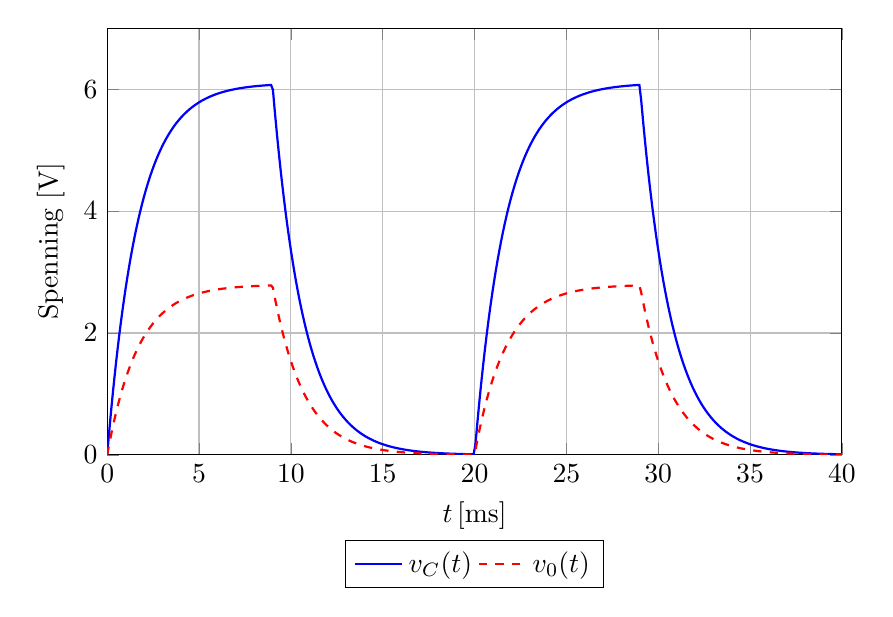
\begin{tikzpicture}
\begin{axis}[
    width=0.9\textwidth,
    height=7cm,
    xlabel={$t\,[\mathrm{ms}]$},
    ylabel={Spenning\ [V]},
    xmin=0, xmax=40,
    ymin=0, ymax=7,
    grid=both,
    legend style={at={(0.5,-0.2)},anchor=north,legend columns=2},
    samples=400
]

    % v_C(t), to perioder via mod(x,20)
    \addplot[
        thick,
        blue,
        domain=0:40
    ]
    {
        (mod(x,20) <= 9) *
            (6.1*(1 - exp(-mod(x,20)/1.69)))
        +
        (mod(x,20) > 9) *
            (6.07*exp(-(mod(x,20)-9)/1.69))
    };
    \addlegendentry{$v_C(t)$}

    % v_0(t) = 0.458 * v_C(t)
    \addplot[
        thick,
        red,
        dashed,
        domain=0:40
    ]
    {
        0.458 *
        (
            (mod(x,20) <= 9) *
                (6.1*(1 - exp(-mod(x,20)/1.69)))
            +
            (mod(x,20) > 9) *
                (6.07*exp(-(mod(x,20)-9)/1.69))
        )
    };
    \addlegendentry{$v_0(t)$}

\end{axis}
\end{tikzpicture}
\caption{Spenningene $v_C(t)$ og $v_0(t)$ over to perioder av inngangssignalet.}
\end{figure}


\subsubsection{Oppladningstida og nedladingstida for $C$}
Siden kondensatoren virkelig trenger uendelig tid for å nå sin maksverdi og uendelig tid for å nå sin minimumsverdi, kan vi bruke en regel. Oppladingstiden er tiden til kondensatoren har nådd ca. 99.3\% og utladingstid er til den har falt til ca. 0.7\% av startverdi. Dette skjer etter omtrent \emph{5 tidskonstanter}.
\[
\begin{aligned}
    t &\approx 5\tau = 5 \cdot 1.69\text{ms}\\
    t &\approx 8.45\text{ms}
\end{aligned}
\]